\documentclass[12pt]{article}
\usepackage[left=1cm, right=1cm, top=2cm,bottom=1.5cm]{geometry} 

\usepackage[parfill]{parskip}
\usepackage[utf8]{inputenc}
\usepackage[T2A]{fontenc}
\usepackage[russian]{babel}
\usepackage{enumitem}
\usepackage[normalem]{ulem}
\usepackage{amsfonts, amsmath, amsthm, amssymb, mathtools,xcolor}
\usepackage{blkarray}

\usepackage{tabularx}
\usepackage{hhline}

\usepackage{accents}
\usepackage{fancyhdr}
\pagestyle{fancy}
\renewcommand{\headrulewidth}{1.5pt}
\renewcommand{\footrulewidth}{1pt}

\usepackage{graphicx}
\usepackage[figurename=Рис.]{caption}
\usepackage{subcaption}
\usepackage{float}

%%Наименование папки откуда забирать изображения
\graphicspath{ {./images/} }

%%Изменение формата для ввода доказательства
\renewcommand{\proofname}{$\square$  \nopunct}
\renewcommand\qedsymbol{$\blacksquare$}

%%Изменение отступа на таблицах
\addto\captionsrussian{%
	\renewcommand{\proofname}{$\square$ \nopunct}%
}
%% Римские цифры
\newcommand{\RN}[1]{%
	\textup{\uppercase\expandafter{\romannumeral#1}}%
}

%% Для удобства записи
\newcommand{\MR}{\mathbb{R}}
\newcommand{\MC}{\mathbb{C}}
\newcommand{\MQ}{\mathbb{Q}}
\newcommand{\MN}{\mathbb{N}}
\newcommand{\MZ}{\mathbb{Z}}
\newcommand{\MTB}{\mathbb{T}}
\newcommand{\MTI}{\mathbb{I}}
\newcommand{\MI}{\mathrm{I}}
\newcommand{\MCI}{\mathcal{I}}
\newcommand{\MJ}{\mathrm{J}}
\newcommand{\MH}{\mathrm{H}}
\newcommand{\MT}{\mathrm{T}}
\newcommand{\MU}{\mathcal{U}}
\newcommand{\MV}{\mathcal{V}}
\newcommand{\MB}{\mathcal{B}}
\newcommand{\MF}{\mathcal{F}}
\newcommand{\MW}{\mathcal{W}}
\newcommand{\ML}{\mathcal{L}}
\newcommand{\MP}{\mathcal{P}}
\newcommand{\VN}{\varnothing}
\newcommand{\VE}{\varepsilon}
\newcommand{\dx}{\, dx}
\newcommand{\dy}{\, dy}
\newcommand{\dz}{\, dz}
\newcommand{\dd}{\, d}


\theoremstyle{definition}
\newtheorem{defn}{Опр:}
\newtheorem{rem}{Rm:}
\newtheorem{prop}{Утв.}
\newtheorem{exrc}{Упр.}
\newtheorem{problem}{Задача}
\newtheorem{lemma}{Лемма}
\newtheorem{theorem}{Теорема}
\newtheorem{corollary}{Следствие}

\newenvironment{cusdefn}[1]
{\renewcommand\thedefn{#1}\defn}
{\enddefn}

\DeclareRobustCommand{\divby}{%
	\mathrel{\text{\vbox{\baselineskip.65ex\lineskiplimit0pt\hbox{.}\hbox{.}\hbox{.}}}}%
}
%Короткий минус
\DeclareMathSymbol{\SMN}{\mathbin}{AMSa}{"39}
%Длинная шапка
\newcommand{\overbar}[1]{\mkern 1.5mu\overline{\mkern-1.5mu#1\mkern-1.5mu}\mkern 1.5mu}
%Функция знака
\DeclareMathOperator{\sgn}{sgn}

%Функция ранга
\DeclareMathOperator{\rk}{\text{rk}}
\DeclareMathOperator{\diam}{\text{diam}}


%Обозначение константы
\DeclareMathOperator{\const}{\text{const}}

\DeclareMathOperator{\codim}{\text{codim}}

\DeclareMathOperator*{\dsum}{\displaystyle\sum}
\newcommand{\ddsum}[2]{\displaystyle\sum\limits_{#1}^{#2}}

%Интеграл в большом формате
\DeclareMathOperator{\dint}{\displaystyle\int}
\newcommand{\ddint}[2]{\displaystyle\int\limits_{#1}^{#2}}
\newcommand{\ssum}[1]{\displaystyle \sum\limits_{n=1}^{\infty}{#1}_n}

\newcommand{\smallerrel}[1]{\mathrel{\mathpalette\smallerrelaux{#1}}}
\newcommand{\smallerrelaux}[2]{\raisebox{.1ex}{\scalebox{.75}{$#1#2$}}}

\newcommand{\smallin}{\smallerrel{\in}}
\newcommand{\smallnotin}{\smallerrel{\notin}}

\newcommand*{\medcap}{\mathbin{\scalebox{1.25}{\ensuremath{\cap}}}}%
\newcommand*{\medcup}{\mathbin{\scalebox{1.25}{\ensuremath{\cup}}}}%

\makeatletter
\newcommand{\vast}{\bBigg@{3.5}}
\newcommand{\Vast}{\bBigg@{5}}
\makeatother

%Промежуточное значение для sup\inf, поскольку они имеют разную высоту
\newcommand{\newsup}{\mathop{\smash{\mathrm{sup}}}}
\newcommand{\newinf}{\mathop{\mathrm{inf}\vphantom{\mathrm{sup}}}}

%Скалярное произведение
\newcommand{\inner}[2]{\left\langle #1, #2 \right\rangle }
\newcommand{\linsp}[1]{\left\langle #1 \right\rangle }
\newcommand{\linmer}[2]{\left\langle #1 \vert #2\right\rangle }

%Подпись символов снизу
\newcommand{\ubar}[1]{\underaccent{\bar}{#1}}

%% Шапка для букв сверху
\newcommand{\wte}[1]{\widetilde{#1}}
\newcommand{\wht}[1]{\widehat{#1}}

%%Трансформация Фурье
\newcommand{\fourt}[1]{\mathcal{F}\left(#1\right)}
\newcommand{\ifourt}[1]{\mathcal{F}^{-1}\left(#1\right)}

%%Символ вектора
\newcommand{\vecm}[1]{\overrightarrow{#1\,}}

%%Пространстов матриц
\newcommand{\mat}[2]{\operatorname{Mat}_{#1\times #2}}

%Оператор для действ и мнимых чисел
\DeclareMathOperator{\IM}{\operatorname{Im}}
\DeclareMathOperator{\RE}{\operatorname{Re}}
\DeclareMathOperator{\li}{\operatorname{li}}


%%Взятие в скобки, модули и норму
\newcommand{\parfit}[1]{\left( #1 \right)}
\newcommand{\modfit}[1]{\left| #1 \right|}
\newcommand{\sqparfit}[1]{\left\{ #1 \right\}}
\newcommand{\normfit}[1]{\left\| #1 \right\|}

%%Функция для обозначения равномерной сходимости по множеству
\newcommand{\uconv}[1]{\overset{#1}{\rightrightarrows}}
\newcommand{\uconvm}[2]{\overset{#1}{\underset{#2}{\rightrightarrows}}}


%%Функция для обозначения нижнего и верхнего интегралов
\def\upint{\mathchoice%
	{\mkern13mu\overline{\vphantom{\intop}\mkern7mu}\mkern-20mu}%
	{\mkern7mu\overline{\vphantom{\intop}\mkern7mu}\mkern-14mu}%
	{\mkern7mu\overline{\vphantom{\intop}\mkern7mu}\mkern-14mu}%
	{\mkern7mu\overline{\vphantom{\intop}\mkern7mu}\mkern-14mu}%
	\int}
\def\lowint{\mkern3mu\underline{\vphantom{\intop}\mkern7mu}\mkern-10mu\int}

%%След матрицы
\DeclareMathOperator*{\tr}{tr}

\makeatletter
\renewcommand*\env@matrix[1][*\c@MaxMatrixCols c]{%
	\hskip -\arraycolsep
	\let\@ifnextchar\new@ifnextchar
	\array{#1}}
\makeatother


%% Переопределение функции хи, чтобы выглядела более приятно
\makeatletter
\@ifdefinable\@latex@chi{\let\@latex@chi\chi}
\renewcommand*\chi{{\@latex@chi\smash[t]{\mathstrut}}} % want only bottom half of \mathstrut
\makeatletter

\begin{document}
\lhead{Математический анализ - \RN{2}}
\chead{Косухин О.Н.}
\rhead{Семинар - 7}

\section*{Интегрирование трансцендентных функций}

\begin{problem}(\textbf{Д2066})
	$$
		\dint P(x)e^{ax}dx
	$$
\end{problem}
\begin{proof}
	Поскольку функции разнородные, то будем интегрировать по частям.
	$$
		e^{ax} = \left(\dfrac{e^{ax}}{a}\right)' \Rightarrow \dint P(x)e^{ax}dx = e^{ax}{\cdot}\dfrac{P(x)}{a} - \dfrac{1}{a}\dint P'(x)e^{ax}dx
	$$
	То есть, мы получили шаг индукции. Тогда можем получить общую формулу:
	$$
		\dint P(x)e^{ax}dx = e^{ax}{\cdot}\left(\dfrac{P(x)}{a} - \dfrac{P'(x)}{a^2} + \dfrac{P''(x)}{a^3} - \dotsc + \dfrac{(-1)^n P^{(n)}(x)}{a^{n+1}}\right) + C
	$$
\end{proof}

Нам удобно интегрировать функции, зависящие от действительной переменной, но принимающая значения в комплексной плоскости:
$$
	F \colon \MR \to \MC, \, F(x) = f(x) + ig(x) \Rightarrow F'(x) = f'(x) + ig'(x)
$$
$$
	\dint F(x) dx = \dint f(x) dx + i\dint g(x) dx 
$$
Мы проверяли следующее:
$$
	e^{(\alpha + i \beta)x} = e^{\alpha x}{\cdot}e^{i\beta x} = e^{\alpha x}(\cos{\beta x} + i \sin{\beta x}) \Rightarrow 
$$
$$	
	\Rightarrow \RE{\left(e^{(\alpha + i \beta)x}\right)} = e^{\alpha x}\cos{\beta x}, \, \IM{\left(e^{(\alpha + i \beta)x}\right)} = e^{\alpha x}\sin{\beta x}
$$
Посчитаем производную у каждой части экспоненты:
$$
	\left(\RE{\left(e^{(\alpha + i \beta)x}\right)}\right)' = e^{\alpha x}\left(\alpha \cos{\beta x}  - \beta \sin{\beta x}\right), \, 
$$
$$
	\left(\IM{\left(e^{(\alpha + i \beta)x}\right)}\right)' = e^{\alpha x}\left(\alpha \sin{\beta x} + \beta \cos{\beta x}\right)
$$
тогда:
$$
	\left(e^{(\alpha + i \beta)x}\right)' = e^{\alpha x}\left(\alpha \cos{\beta x}  - \beta \sin{\beta x}\right) + i e^{\alpha x}\left(\alpha \sin{\beta x} + \beta \cos{\beta x}\right) = (\alpha + i \beta){\cdot}e^{(\alpha + i\beta)x}
$$
Таким образом, для интеграла эти же правила будут работать $\Rightarrow$ формула из задачи $2066$ будет работать и тогда, когда число $a$ - комплексное.
\begin{problem}(\textbf{Д2067}) (только одна часть)
	$$
		\dint P(x) \cos{(ax)} dx
	$$
\end{problem}
\begin{proof}
	Снова будем интегрировать по частям:
	$$
		\dint P(x) \cos{(ax)} dx = \sin{(ax)}{\cdot} \dfrac{P(x)}{a} - \dfrac{1}{a}\dint P'(x) {\cdot}\sin{(ax)}dx 
	$$
	Проинтегрируем по частям ещё раз:
	$$	
		\sin{(ax)}{\cdot} \dfrac{P(x)}{a} - \dfrac{1}{a}\dint P'(x) {\cdot}\sin{(ax)}dx  = \sin{(ax)}{\cdot} \dfrac{P(x)}{a} + \cos{(ax)}{\cdot}\dfrac{P'(x)}{a^2} - \dfrac{1}{a^2}\dint P''(x)\cos{(ax)} dx
	$$
	Таким образом, мы получили шаг индукции и формула итоговая будет выглядеть так:
	$$
		\dint P(x) \cos{(ax)} dx = \dfrac{\sin{(ax)}}{a}{\cdot}\left( P(x) - \dfrac{P''(x)}{a^2} + \dfrac{P^{(4)}(x)}{a^4} - \dotsc + (-1)^k \dfrac{P^{(2k)}(x)}{a^{2k} }\right) + 
	$$
	$$
		+ \dfrac{\cos{(ax)}}{a^2}\left(P'(x) - \dfrac{P'''(x)}{a^2} + \dotsc + \dfrac{(-1)^m P^{(2m+1)}(x)}{a^{2m}}\right) + C
	$$
	где $k = \left[\tfrac{n}{2}\right]$ и $m = \left[\tfrac{n-1}{2}\right]$ - такое, чтобы $2m +1 < n$. Также заметим, что:
	$$
		\dint P(x) \cos{(ax)} dx = \RE\left(\dint P(x) e^{iax}dx \right)
	$$
	поскольку косинус можно связать с комплексными экспонентами следующим образом:
	$$
		\cos{(ax)} = \RE(e^{iax}) \vee \cos{(ax)} = \dfrac{1}{2}(e^{iax} + e^{-iax})
	$$
	Таким образом, можно взять разложение экспоненты и взять действительную часть:
	$$
		\dint P(x)e^{iax}dx = e^{iax}{\cdot}\left(\dfrac{P(x)}{ia} + \dfrac{P'(x)}{a^2} - \dfrac{P''(x)}{ia^3} - \dotsc + \dfrac{(-1)^n P^{(n)}(x)}{(ia)^{n+1}}\right) + C = 
	$$
	$$
		=(\cos{(ax)} + i \sin{(ax)}){\cdot}\left(\dfrac{P(x)}{ia} + \dfrac{P'(x)}{a^2} - \dfrac{P''(x)}{ia^3} - \dotsc + \dfrac{(-1)^n P^{(n)}(x)}{(ia)^{n+1}}\right)  + C
	$$
\end{proof}

Применим результаты теоретических задач, решенных выше.
\begin{problem}(\textbf{Д2068})
	$$
		\dint x^3 e^{3x}dx
	$$
\end{problem}
\begin{proof}
	$$
		\dint x^3 e^{3x}dx = e^{3x}\left(\dfrac{x^3}{3} - \dfrac{3x^2}{3^2} + \dfrac{6x}{3^3} - \dfrac{6}{3^4}\right) + C
	$$
\end{proof}
\begin{problem}(\textbf{Д2076})
	$$
		\dint x e^x \sin{x} dx
	$$
\end{problem}
\begin{proof}
	Заметим, что $e^x \sin{x} = \IM{(e^x (\cos{x} + i\sin{x}))} = \IM(e^{(1 + i)x})$, следовательно:
	$$
		\dint x e^x \sin{x} dx = \IM\left(\dint x e^{(1 + i)x}dx\right) = \IM \left(e^{(1 + i)x} \left( \dfrac{x}{1 + i} - \dfrac{1}{(1 + i)^2}\right) + C\right)
	$$
	$$
		e^{(1 + i)x} \left( \dfrac{x}{1 + i} - \dfrac{1}{(1 + i)^2}\right) = (e^x\cos{x} + ie^{x}\sin{x}){\cdot}\left(\dfrac{x(1 - i)}{2} - \dfrac{(1-i)^2}{4}\right)= 
	$$
	$$
		=(e^x\cos{x} + ie^{x}\sin{x}){\cdot}\left( \dfrac{x - xi}{2} - \dfrac{1 - 2i -1}{4}\right) =(e^x\cos{x} + ie^{x}\sin{x}){\cdot}\left(\dfrac{x - xi}{2} + \dfrac{ i}{2}\right) = 
	$$
	$$
		 = e^x\cos{x}{\cdot}\dfrac{x}{2} + e^x \sin{x}{\cdot}\dfrac{(x-1)}{2}  +  i{\cdot}\left(e^x \cos{x}{\cdot}\dfrac{(1- x)}{2} + e^{x}\sin{x}{\cdot}\dfrac{x}{2} \right) \Rightarrow
	$$
	$$
		\Rightarrow \IM\left(\dint x e^{(1 + i)x}dx\right) = e^x \cos{x}{\cdot}\dfrac{(1- x)}{2} + e^{x}\sin{x}{\cdot}\dfrac{x}{2} + C
	$$	
\end{proof}
\begin{rem}
	Заметим, что задачу можно было решить только методом интегрирования по частям, но это было бы сложнее.
\end{rem}

\subsection*{Короткое напоминание про комплексные числа}
$$
	z = x + iy = r{\cdot}(\cos{\varphi} + i\sin{\varphi}) = r{\cdot}e^{ i\varphi}, \, \RE{(z)} = x, \, \IM{(z)} = y
$$
\begin{figure}[H]
	\centering
	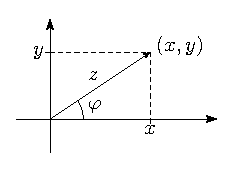
\includegraphics[width=0.25\textwidth]{MA2S7_1.eps}
	\caption{Визуализация комплексного числа.}
	\label{7_1}
\end{figure}
$$
	e^{\alpha + i\beta} = e^{\alpha}{\cdot}(e^{i\beta}) = e^{\alpha}{\cdot}(\cos{\beta} + i\sin{\beta})
$$
$$
	e^{i\beta_1}{\cdot}e^{i\beta_2} = e^{i(\beta_1 + \beta_2)}
$$
В следующем семестре мы докажем:
$$
	e^{x} = 1 + x + \dfrac{x^2}{2!} + \dotsc + \dfrac{x^n}{n!} + \dotsc
$$
Обобщение для комплексных чисел будет выглядеть так:
$$
	e^z = 1 + z + \dfrac{z^2}{2!} + \dotsc  + \dfrac{z^n}{n!} + \dotsc
$$
Если записать ряды для косинуса и синуса, то мы будем иметь:
$$
	\cos{x} = 1 - \dfrac{x^2}{2!} + \dfrac{x^4}{4!} - \dotsc 
$$
$$
	\sin{x} = x - \dfrac{x^3}{3!} + \dfrac{x^5}{5!} - \dotsc
$$
Если мы просуммируем ряд косинуса и ряд синуса, умноженный на $i$, то мы получим ряд $e^{ix}$:
$$
	\cos{x} + i\sin{x} = 1 + ix - \dfrac{x^2}{2!} - i\dfrac{x^3}{3!} + \dfrac{x^4}{4!} + i\dfrac{x^5}{5!} - \dotsc = e^{ix} = 1 + ix + \dfrac{(ix)^2}{2!} +\dfrac{(ix)^3}{3!} + \dotsc 
$$

\begin{problem}(\textbf{Д2073})
	$$
		\dint x^2 e^{\sqrt{x}} dx
	$$
\end{problem}
\begin{proof}
	Сделаем замену $t = \sqrt{x}$, тогда:
	$$
		x = t^2, \, dx = 2tdt 
	$$
	$$
		\dint x^2 e^{\sqrt{x}} dx = \dint t^4 e^t 2t dt = 2 \dint e^t t^5 = 2e^t\left(t^5 - 5t^4 + 20t^3 - 60t^2 + 120t - 120\right) + C, \, t = \sqrt{x}
	$$
\end{proof}
Заметим, в похожих задачах с синусами или косинусами надо понижать степень, например:
$$
	\cos^2{bx} = \dfrac{1 + \cos{2bx}}{2}, \, \sin{(3x)} = 3\sin{x} - 4\sin^3{x} \Rightarrow \sin^3{x} = \dfrac{ 3\sin{x} - \sin{(3x)} }{4}
$$
Таким образом, похожие задачи решаются одними формулами с многочленами выше, но чтобы к ним свести надо либо использовать комплексные числа, либо интегрировать по частям, либо делать замены переменной, либо тригонометрические преобразования.

\subsection*{Интегралы с экспонентами}
\begin{problem}(\textbf{Д2082})
	$$
		\dint \dfrac{dx}{(1 + e^x)^2}
	$$
\end{problem}
\begin{proof}
	Сделаем замену переменных:
	$$
		t =e^x, \, x = \ln{t},\, dx = \dfrac{dt}{t}
	$$
	$$
		\dint \dfrac{dx}{(1 + e^x)^2} = \dint \dfrac{dt}{t(1 +t)^2} = \dint \dfrac{A}{t} + \dfrac{B}{t + 1} + \dfrac{C}{(t+1)^2} dt = \dint \dfrac{A(t+1)^2 + Bt(t+1) + Ct}{t(t+1)^2}dt
	$$
	Заметим, что если снизу линейные множители, то сверху просто константа, поскольку ориентация на степень множителя, а не на общую степень.
	$$
		A = 1, \, A + B = 0 \Rightarrow B = -1, \, 2A + B + C = 0 \Rightarrow C= -1
	$$
	$$
		 \dint \dfrac{A}{t} + \dfrac{B}{t + 1} + \dfrac{C}{(t+1)^2} dt = \ln{t} - \ln{(t +1)} - \dfrac{1}{t + 1} + C = x - \ln{(e^x + 1)} - \dfrac{1}{e^x + 1} +C
	$$
\end{proof}

\begin{problem}(\textbf{Д2087})
	$$
		\dint\dfrac{dx}{\sqrt{e^x - 1}}
	$$
\end{problem}
\begin{proof}
	Сделаем замену переменных (уберем то, что не очень нравится):
	$$
		t = \sqrt{e^x - 1} \Rightarrow t^2 = e^x - 1 \Rightarrow x = \ln{(1 +t^2)}, \, dx = \dfrac{2t}{1 + t^2}dt
	$$
	$$
		\dint\dfrac{dx}{\sqrt{e^x - 1}} = \dint \dfrac{2t}{1+t^2}{\cdot}\dfrac{1}{t}dt = 2 \arctg{t} + C = 2 \arctg{(\sqrt{e^x - 1})} +C
	$$
\end{proof}
В таких задачах часто надо сделать просто правильную замену. Но оказывается, что могут появляться и неберущиеся интегралы, то есть они не выражаются через элементарные функции. Введём функцию \uwave{интегрального логарифма}:
$$
	\li(x) = \dint \dfrac{dx}{\ln{x}}
$$
с той поправкой, что справа стоит множество функций и мы берём конкретного представителя. Рассмотрим следующую задачу.
\begin{problem}(\textbf{Д2091})
	$$
		\dint R(x) e^{ax} dx, \, R(x) = \dfrac{P(x)}{(x - x_1)^{k_1}{\cdot}\dotsc(x - x_m)^{k_m}}
	$$
	$R(x)$ - рациональная функция, знаменатель которой имеет лишь действительные корни. Необходимо показать, что такой интеграл выражается через элементарные функции и $\li(e^{ax})$.
\end{problem}
\begin{proof}
	Мы знаем, что для вида $R(x)$ есть разложение на простейшие дроби:
	$$
		R(x) = \dfrac{P(x)}{(x - x_1)^{k_1}{\cdot}\dotsc(x - x_m)^{k_m}} = \dfrac{A_1}{x - x_1} + \dfrac{A_2}{(x-x_1)^2} + \dotsc + \dfrac{A_{k_1}}{(x - x_1)^{k_1}} + \dotsc
	$$
	Если мы научимся интегрировать $e^{ax}\dfrac{A_k}{(x - x_i)^k}$, то тогда мы сможем интегрировать всё выражение. 
	$$
		\forall k \geq 2, \, \dfrac{1}{(x-b)^k} = \left(\dfrac{1}{(x - b)^{k-1}(1 -k)}\right)' \Rightarrow
	$$
	$$
		\Rightarrow \dint \dfrac{e^{ax}}{(x - b)^k}dx = \dfrac{1}{1 -k}{\cdot}\dfrac{e^{ax}}{(x - b)^{k-1}} - \dfrac{1}{1 -k} \dint \dfrac{e^{ax}}{(x - b)^{k-1}}dx
	$$
	Следовательно, можно интегрировать по индукции до тех пор, пока не остановимся на функции:
	$$
		\dint \dfrac{e^{ax}}{x - b}dx = |t = x - b| = \dint\dfrac{e^{a(t + b)}}{t}dt = e^{ab}\dint\dfrac{e^{at}}{t}dt = \left|y = e^{at}, \, t = \dfrac{1}{a}\ln{y}, \, dt = \dfrac{1}{y}dy \right| = 
	$$
	$$
		=e^{ab}\dint \dfrac{y}{\tfrac{1}{a}\ln{y}}{\cdot}\dfrac{1}{ay}dy = e^{ab}\dint \dfrac{dy}{\ln{y}} = e^{ab}\li(y) + C = e^{ab}\li\left(e^{a(x - b)}\right) + C
	$$
\end{proof}

\subsection*{Интегрирование по частям}

\begin{problem}(\textbf{Д2098})
	$$
		\dint \ln^n{x}dx
	$$
\end{problem}
\begin{proof}
	Вспомним, что мы считали такой интеграл для $n=1$:
	$$
		\dint \ln{x} dx = x{\cdot}\ln{x} - \dint x{\cdot}\dfrac{1}{x}dx = x\ln{x} - x + C
	$$
	В общем случае:
	$$
		\MI_n = \dint \ln^n{x}dx = \dint 1{\cdot}\ln^n{x}dx = x \ln^{n}{x} - \dint x{\cdot}n{\cdot}\ln^{n-1}{x}{\cdot}\dfrac{1}{x}dx = 
	$$
	$$
		= x \ln^{n}{x} - \dint n{\cdot}\ln^{n-1}{x}dx = x \ln^{n}{x} - n{\cdot}\MI_{n-1} \Rightarrow
	$$
	$$
		\Rightarrow \MI_n = x \ln^n{x} - n\left(x \ln^{n-1}{x} - (n-1){\cdot}\left(x\ln^{n-2}{x} - \dotsc \right)\right) = 
	$$
	$$	
		= x\ln^n{x} - nx\ln^{n-1}{x} + n(n-1)x\ln^{n-2}{x} - \dotsc + (-1)^nn!x + C
	$$
	Далее можно проверить это выражение по индукции. Базу уже проверяли, сделать шаг индукции и проверить, что выполняется реккурентное соотношение.
\end{proof}

\begin{problem}(\textbf{Д2110})
	$$
		\dint \arcsin{\left(\dfrac{2\sqrt{x}}{1 + x}\right)}dx
	$$
\end{problem}
\begin{proof}
	Проинтегрируем выражение по частям:
	$$
		\dint 1{\cdot}\arcsin{\left(\dfrac{2\sqrt{x}}{1 + x}\right)}dx = x{\cdot}\arcsin{\left(\dfrac{2\sqrt{x}}{1 + x}\right)} - \dint x{\cdot}\dfrac{1}{\sqrt{1 - \tfrac{4x}{(1 +x)^2}}}{\cdot}   \dfrac{\tfrac{1}{\sqrt{x}}(1+x) - 2\sqrt{x}}{(1 + x)^2}dx = 
	$$
	$$
		=	x{\cdot}\arcsin{\left(\dfrac{2\sqrt{x}}{1 + x}\right)} - \dint \dfrac{1 + x}{|1 -x|}{\cdot}\dfrac{(1 - x)\sqrt{x}}{(1 + x)^2}dx = x{\cdot}\arcsin{\left(\dfrac{2\sqrt{x}}{1 + x}\right)} - \dint \dfrac{\pm\sqrt{x}}{(1 + x)}dx
	$$
	Если $x \in [0,1) \Rightarrow +, \, x \in [1,+\infty) \Rightarrow -$. Сделаем замену:
	$$
		\dint \dfrac{\sqrt{x}dx}{1 + x} = \left|\sqrt{x} = t, \, x = t^2, \, dx = 2t dt\right| = \dint \dfrac{2t^2}{1 +t^2}dt = 2t - 2\dint\dfrac{1}{1 + t^2}dt = 2\sqrt{x} - 2\arctg{\sqrt{x}} + C \Rightarrow
	$$
	$$
		\Rightarrow \dint \arcsin{\left(\dfrac{2\sqrt{x}}{1 + x}\right)}dx = x{\cdot}\arcsin{\left(\dfrac{2\sqrt{x}}{1 + x}\right)} \mp 2\left(\sqrt{x} - \arctg{\sqrt{x}}\right) + C
	$$
	Также можно было сделать немного другое интегрирование по частям:
	$$
		\dint 1{\cdot}\arcsin{\left(\dfrac{2\sqrt{x}}{1 + x}\right)}dx = ( x+1){\cdot}\arcsin{\left(\dfrac{2\sqrt{x}}{1 + x}\right)} - \dint (x+1){\cdot}\dfrac{1}{\sqrt{1 - \tfrac{4x}{(1 +x)^2}}}{\cdot}   \dfrac{\tfrac{1}{\sqrt{x}}(1+x) - 2\sqrt{x}}{(1 + x)^2}dx = 
	$$
	$$
		=	(x+1){\cdot}\arcsin{\left(\dfrac{2\sqrt{x}}{1 + x}\right)} - \dint \dfrac{1 + x}{|1 -x|}{\cdot}\dfrac{(1 - x)}{\sqrt{x}(1 + x)}dx = (x+1){\cdot}\arcsin{\left(\dfrac{2\sqrt{x}}{1 + x}\right)} \mp \dint \dfrac{1}{\sqrt{x}}dx=
	$$
	$$
		=	(x+1){\cdot}\arcsin{\left(\dfrac{2\sqrt{x}}{1 + x}\right)} \mp 2\sqrt{x} + C
	$$
\end{proof}
\begin{problem}(\textbf{Д2113})
	$$
		\dint x\arctg{x}{\cdot}\ln{(1 + x^2)}dx
	$$
\end{problem}
\begin{proof}
	Вспомним, как решать следующую задачу:
	$$
		\dint x\arctg{x}dx = \dfrac{x^2}{2}\arctg{x} - \dfrac{1}{2}\dint\dfrac{x^2}{1 + x^2}dx = \dfrac{x^2}{2}\arctg{x} - \dfrac{x}{2} + \dfrac{1}{2}\arctg{x} + C
	$$
	Проинтегрируем по частям исходное выражение:
	$$
		\dint x\arctg{x}{\cdot}\ln{(1 + x^2)}dx = \left(\dfrac{x^2}{2}\arctg{x} - \dfrac{x}{2} + \dfrac{1}{2}\arctg{x}\right){\cdot}\ln{(1 + x^2)} -
	$$
	$$
		-\dfrac{1}{2}\dint \left( (x^2 + 1)\arctg{x} - x \right)\dfrac{2x}{1 + x^2}dx
	$$
	$$
		\dfrac{1}{2}\dint \left( (x^2 + 1)\arctg{x} - x \right)\dfrac{2x}{1 + x^2}dx = \dint x\arctg{x}dx - \dint \dfrac{x^2}{1 +x^2}dx 
	$$
	То есть интегралы, которые только что посчитали.
\end{proof}

\begin{problem}(\textbf{Д2165})
	$$
		\dint \dfrac{1 + \sin{x}}{1 + \cos{x}}e^x dx
	$$
\end{problem}
\begin{proof}
	Попробуем упростить дробь с помощью формул половинного угла:
	$$
		\sin{x} = 2 \sin{\tfrac{x}{2}}\cos{\tfrac{x}{2}} \Rightarrow 1 + \sin{x} = \sin^2{\tfrac{x}{2}} + \cos^2{\tfrac{x}{2}} + 2 \sin{\tfrac{x}{2}}\cos{\tfrac{x}{2}} = \left(\sin{\tfrac{x}{2}} + \cos{\tfrac{x}{2}}\right)^2 
	$$
	$$
		\cos{x} = 2 \cos^2 \tfrac{x}{2} - 1 \Rightarrow 1 + \cos{x} = 2 \cos^2 \tfrac{x}{2}
	$$
	Похоже, что это не сильно поможет и надо интегрировать по частям (решение со следующего семинара):
	$$
		\dint \dfrac{1 + \sin{x}}{1 + \cos{x}}e^x dx = \dfrac{1 + \sin{x}}{1 + \cos{x}}e^x - \dint e^x\dfrac{\cos{x}(1 + \cos{x}) + (1 + \sin{x})\sin{x}}{(1 + \cos{x})^2}dx 
	$$
	$$
		\dint e^x\dfrac{\cos{x}(1 + \cos{x}) + (1 + \sin{x})\sin{x}}{(1 + \cos{x})^2}dx = \dint e^x\dfrac{1 + \cos{x}  + \sin{x} }{(1 + \cos{x})^2}dx \Rightarrow
	$$
	$$
		\Rightarrow \dfrac{1 + \cos{x}  + \sin{x} }{(1 + \cos{x})^2} = \dfrac{1}{1 + \cos{x}} + \dfrac{\sin{x}}{(1 + \cos{x})^2} = \dfrac{1}{1 + \cos{x}} + \left(\dfrac{1}{1 + \cos{x}}\right)' \Rightarrow 
	$$
	$$
		\Rightarrow \left( e^x\dfrac{1 + \cos{x}  + \sin{x} }{(1 + \cos{x})^2}\right)' = \dfrac{e^x}{1 + \cos{x}} + e^x\left(\dfrac{1}{1 + \cos{x}}\right)' \Rightarrow 
	$$
	$$
		\Rightarrow \dint \dfrac{1 + \sin{x}}{1 + \cos{x}}e^x dx = e^x\dfrac{\sin{x}}{1 + \cos{x}} + C
	$$
\end{proof}
\begin{rem}
	Как получилось додуматься до решения? Заметели следующее:
	$$
		\dfrac{1 + \cos{x} + \sin{x} + \sin{x}\cos{x}}{(1 + \cos{x})^2} = \dfrac{(1 + \cos{x})(1 + \sin{x})}{(1 + \cos{x})^2}
	$$	
	Обозначим:
	$$
		\MI = \dint \dfrac{1 + \sin{x}}{1 + \cos{x}}e^x dx \Rightarrow \dint e^x\dfrac{\cos{x}(1 + \cos{x}) + (1 + \sin{x})\sin{x}}{(1 + \cos{x})^2}dx = \MI - \dint\dfrac{\sin{x}\cos{x}}{(1 + \cos{x})}e^xdx 
	$$
	А дальше накидывать производную на дробь - не очень хорошая идея, поскольку будет нарастать знаменатель, поэтому логично было бы убрать производную отсюда. Тогда выделяя множитель:
	$$
		\dfrac{\sin{x}}{(1 + \cos{x})^2} = \left(\dfrac{1}{1 + \cos{x}}\right)'
	$$
	Следовательно, производная перебрасывается на $e^x \cos{x}$, тогда снова появляется $\MI$ и сокращается.
\end{rem}

\textbf{ДЗ}: В этот раз без конкретики, но были заданы упражнения $2077$, $2093$.

\end{document}